%%%%%%%%%%%%%%%%%%%%%%%%%%%%
% Two Sword Lengths Apart
% 10 December 2014
%%%%%%%%%%%%%%%%%%%%%%%%%%%%

% !Rnw weave = knitr

\documentclass[a4paper]{article}
\usepackage{fullpage}
\usepackage{lscape}
\usepackage[authoryear]{natbib}
\usepackage{setspace}
    \doublespacing
\usepackage{hyperref}
\hypersetup{
    colorlinks,
    citecolor=black,
    filecolor=black,
    linkcolor=cyan,
    urlcolor=cyan
}
\usepackage{booktabs}
\usepackage{dcolumn}
\usepackage{url}
\usepackage{tikz}
\usepackage{todonotes}
\usepackage{verbatim}
\usepackage{endnotes}
\usepackage{graphicx}

\usepackage[margins]{trackchanges}


\setlength{\belowcaptionskip}{0.5cm}

%%%%%%% Title Page %%%%%%%%%%%%%%%%%%%%%%%%%%%%%%%%%%%%%%%%%%%%
\title{Two Sword Lengths Apart: Credible Commitment Problems and Physical Violence in Multi-party Elected National Legislatures}

\author{Christopher Gandrud \\
                {\emph{Hertie School of Governance}}\footnote{Post-doctoral Researcher. Friedrichstra{\ss}er 180. 10117 Berlin, Germany. Email: \href{mailto:gandrud@hertie-school.org}{gandrud@hertie-school.org}. Thank you to Gary Cox, Simon Hix, Shirin Rai, Carole Spary, as well as seminar participants at the Hertie School of Governance and Yonsei University for very helpful comments and insights. I would also like to thank Hortense Badarani for excellent research assistance and my students at the LSE for inspiration. Full replication files--including data and source code--can be found at \url{https://github.com/christophergandrud/leg_violence_paper1}. An earlier version was circulated under the title ``Two Sword Lengths: Losers' consent and violence in national legislatures''.}}

\begin{document}

\maketitle

%%%%%%% Abstract %%%%%%%%%%%%%%%%%%%%%%%%%%%%%%%%%%%%%%%%%%%%
\begin{abstract}
Multi-party elected national legislatures should be venues for peacefully resolving conflicts between opposing groups. However, they can become scenes of physical violence. Such violence is an indication that a country's legislative institutions are functioning far from perfectly as legislative actors are deciding to disregard the rules of the game. In some cases, such as recently in Ukraine, violence can indicate and possibly fuel deeper political divisions. In this first global study of legislative violence, I show that brawls are more likely when legislators find it difficult to credibly commit to follow peaceful bargains. Credible commitment problems are more acute in countries with disproportionate electoral outcomes and in new democracies. I find robust evidence for this argument using a case study of legislative violence in the antebellum United States Senate and a new global data set.
\end{abstract}


\paragraph{Keywords:} legislatures, violence, credible commitment problems, electoral proportionality, institutional design, majority and minority governments

\vspace{0.3cm}

%%%%%%% Introduction %%%%%%%%%%%%%%%%%%%%%%%%%%%%%%%%%%%%%%%%%%%%

Though legislators in democracies are often described as `battling' or `fighting' we expect these battles to be in terms of rhetoric and procedural manoeuvres, circumscribed by non-violent rules, that culminate in votes. The outcomes of these contests are then respected by all legislators. However, metaphorical battles sometimes become physical fights between members of legislatures.

Many legislatures' histories contain incidents of physical violence between legislators. In 1856 a member of the United States House of Representatives caned a senator unconscious in the Senate chamber \citep{USSenateCanning}. It has been suggested that the United Kingdom's House of Commons is physically designed to prevent violence between members. The Government and Opposition benches are said to be ``two sword lengths apart" \citep{ParliamentUKSword} so that duels will be fought with words rather than swords. Actual, sword fights do not seem to have taken place in the Commons chamber, but violent incidences did occur in the 1800s \citep[see][]{ByrneViolence}. Violence in legislatures continues to occur. Recent instances of violence between legislators include brawls in South Korea in 2009\footnote{See \url{http://dailym.ai/1rHLruX}. Accessed October 2014} and in Ukraine during the years leading up to the civil war.\footnote{For example see \url{http://online.wsj.com/articles/SB10001424052748704471204575209572380473814}. Accessed October 2014} In 2013 a large confrontation happened in the Venezuelan National Assembly when the Assembly President withheld speaking time from legislators who did not recognize president's victory in a very highly contested election.\footnote{See \url{http://edition.cnn.com/2013/04/30/world/americas/venezuela-lawmakers-violence/index.html}. Accessed October 2014.}

Physical violence is a dramatic break from scholars' assumption that compliance with legislative rules of the game is a given and as such symbolizes poorly functioning legislative institutions. Some work has examined the strategic and expressive choices politicians make when they decide not to participate in the democratic rules of the game \citep{wilkinson2006,Beaulieu2008,BeaulieuForthcoming}. In this paper I extend this work by advancing a theory of legislative violence in multi-party elected national legislatures and test it using both case study and global-level data. Indeed, this paper includes the first cross-country description of violence between legislators. It also provides us with an important window for understanding what makes legislatures work (or not) as institutions for peacefully resolving disputes between opposing parties.\footnote{Note that the underlying process I discuss that creates conditions for violence likely also creates environments where legislators use other types of less violent--and less easily observable on a global scale--forms of legislative rule breaking.}

I begin the paper by advancing an argument for understanding when legislative violence between members of multi-party elected legislatures is more likely. Though legislators' personalities surely play some part in any given violent incident, I argue that the probability of violence is strongly influenced by the wider political environment. In particular, violence is much more likely when there are \emph{credible commitment problems} that incentivize legislators to break peaceful bargains. At least two observable institutional factors are important for affecting the likelihood that commitments will be adhered to: the \emph{proportionality of a country's electoral outcomes} and the \emph{age of its democracy}. After proposing this argument and discussing a number of key alternative explanations, I begin to empirically examine it with a case study of violence in the antebellum United States Senate. I then move to a global level study of contemporary legislative violence by describing a new data set of legislative violence. In this section I also demonstrate simple associations between my argument's key variables and violence on a global scale. I then discuss the variables and parametric regression models I use to further study these events. Finally, I lay out the evidence from these models that legislative violence is more prevalent in countries with disproportionate electoral outcomes and in new democracies. I also find that violence is more likely in legislatures with small minority governments. I conclude the paper with a discussion of the possible implications of these findings for democratic institution designers and directions for future research.

%%%%%%%%%%%%%%%%%%%%%%%%%%%%%%%%%%%%%%%%%%%%%% Previous Research & Framework

\section{Understanding Legislative Violence}

Legislative violence, like other forms of violent disruption \citep[see][]{Beaulieu2008,BeaulieuForthcoming,wilkinson2006}, could be used for strategic purposes by both legislative winners and losers. Legislative losers--those who are not in control of the ``legislative cartel''  that sets the agenda \citep{cox2007} and are not part of the deciding majority--may use violence to stall legislation or rule changes they dislike. Winners--those in the legislative cartel--could use violence to prevent losers from utilizing procedures that might constrain their decision-making power. Both winners and losers may use violence to shore up support among their proponents, as a way of expressing dissatisfaction with legislative outcomes, and to publicize issues they and their supporters care about. Winners may not only use active violence, but also might make a strategic choice not to use their powers, e.g. control of security forces, to prevent or curtail losers' violence with the hope that losers will be publicly discredited.

Just because actors can gain a strategic advantage or express their discontent through violence does not mean they will choose to. Though violence may have strategic benefits, it also entails costs. Violent conflict has physical costs. In a number of incidents legislators have been hospitalized or even, as in the case of Charles Sumner discussed below, almost died. Beyond the physical costs of legislative violence, there may be other costs such as legal penalties and reputational costs.

However, there are situations where legislators perceive the benefits of violence to be greater than the costs. Violence in multi-party elected legislatures is often precipitated by situations where legislators find it difficult to credibly commit to follow peaceful bargaining outcomes. In these situations the perceived benefits of violence can outweigh the costs. \cite{Fearon1995} argued that when actors are not able to make credible commitments the benefits from violent conflict can outweigh the costs making violence more likely \cite[see also][]{Powell2006}. If it is difficult to believe that a peaceful bargaining outcome will actually happen because bargained commitments will likely be broken, actors will choose violence to achieve their goals. This logic is applicable to legislatures. In multi-party elected legislatures winners and losers--who may some day become winners--need to be able to credibly commit to not use or remake legislative procedures in their narrow self-interest. They need to commit to limits on their power \citep{riker1982,Gaubatz1996}, especially legislative rules and procedures that are the result of peaceful bargaining processes. If they are not able to credibly make these commitments then legislators may come to believe that disruption and violence is the best way to achieve their goals, despite its costs. What makes legislative credible commitment problems more or less severe?

Credible commitment problems are generally smaller and therefore violence is less likely when \emph{ seats in the legislature and legislative resources, such as speaking time and committee appointments, proportionally correspond to voters' support}. For simplicity I will refer to such legislatures as `fair'. I argue that a lack of correspondence between legislative power and voter support increases legislative credible commitment problems in at least two ways: it (a) creates possibilities for shifts in power from those who benefit from the status quo to beneficiaries of fairer rules and (b) prevents fairness equilibria.

Unfair legislatures have the possibility for large and rapid shifts in legislative power from those who benefit from the status quo rules to those that would benefit from new rules. For example, if an electoral system that creates disproportionate outcomes becomes more proportional, then the winning parties may be likely to change over the course of one election. The new winners could then further alter legislative procedures to benefit themselves through control of the legislative cartel. \cite{Powell2004,Powell2006} identified major commitment problems in bargains over issues affecting future bargaining power when there could be large and rapid power shifts. We can apply his logic to legislatures. Temporarily weak legislators--those with disproportionately fewer seats and access to legislative resources under the status quo--who are not in the legislative cartel need to `buy off' those that are temporarily strong--the beneficiaries of the status quo in the cartel--in order to avoid the strong changing the rules to further benefit themselves. `Buying off' in this context may simply mean agreeing to continue rules that make the legislature unfair at the status quo level. However, because the presently weak have the potential to be much stronger, they are likely to renege on agreements that disproportionately benefit the temporarily strong. They may also have an incentive to use disruption or violence to prevent further rule changes that limit their power or indeed force the rules to become fairer to actively increase their power. Importantly, in the absence of credible commitments from the temporarily weak, the \emph{temporarily strong may use preemptive violence to prevent the rules from becoming fairer}.

Why do very fair legislatures not create equally large credible commitment problems? Presumably legislators that would benefit from a large increases in unfairness would find it difficult to credibly commit. In other words, why would a fair legislature create an equilibrium? Rabin's \citeyearpar{Rabin1993} work studying bargaining consequences when actors care about fairness in addition to material well-being provides an answer. Because actors care about fairness, they are more likely to maintain commitments (punish defectors), even if it hurts their material well-being, when others are being fair (unfair). One form of punishment could be reputational damage inflicted in fair systems by both supporters and opponents of violent legislators who care about fairness. This reduces legislators' incentives to defect from fair rules and bargains even if they could gain legislative power by increasing unfairness. As such credible commitment problems are lower and actors can reach a ``fairness equilibrium''. Experimental research supports the idea that commitments are more credible if they are fairer \citep{Ellingsen2004} and can even act as an enforcement device for incomplete contracts \citep[see][for a review]{Fehr2008}.

\subsection{Observing Situations Where Credible Commitment Problems are Worse}

To empirically test my theory I focus on two clearly observable institutional factors that structure bargaining by influencing legislators' credible commitment problems: proportionality of electoral outcomes and age of democracy. Please note that these are likely not the only factors that shape credible commitments, but they are definitively observable in a cross-country study.

\paragraph{Proportional Electoral Outcomes}

Possibly the most important and clearly observable component of legislature fairness is the proportionality of the election that allocated its seats and therefore the control of its procedures. Disproportional, i.e. unfair, electoral outcomes create credible commitment problems as they create the potential for shifts in power from beneficiaries of unfair to fair rules. More proportional systems conversely enable fairness equilibria. At what observable levels of disproportionately would we expect to see more violence? At most levels of disproportionately there may be credible commitment problems to some degree, because there will be legislators who benefit from an increase in proportionality. It is only when outcomes are close to perfectly proportional that the gains from increasing proportionality are very small or virtually none existent. At the same time in systems with very proportional electoral outcomes it is easy for all to identify the electoral outcomes as fair, thus enabling fairness equilibria.\footnote{When there is ambiguity over how fair the system is actors may not impose very high costs, such as reputational damage, for breaking the rules.} Because of this we should not expect a linear relationship between disproportionately and violence. There should instead be a threshold effect where very proportional electoral outcomes will have very low levels of violence due to very small or non-existent credible commitment problems.

Recent empirical research on the functional form of the relationship between political trust and disproportionality provides some initial evidence for the claim that there could be a threshold effect between disproportionality and legislative violence. \cite{Marien2011} found that there was a curvilinear relationship between proportional electoral outcomes and citizens' political trust. Feelings of political trust were highest with very proportional outcomes as well as disproportional or majoritarian systems. Countries in the middle had the lowest trust. Marien argues that high trust in very proportional systems is caused by high fairness. The fairness effect seems to quickly disappear as we move in the direction of more disproportionate outcomes. Marien argues that high voter trust in very disproportionate countries is caused not by fairness, but by high accountability. So should we expect a similar curvilinear relationship between proportionality and legislative violence? Probably not. Though accountability may please voters in general, there is little reason to believe that this will ameliorate the credible commitment problems among legislators created by unfairness.

For these reasons \emph{we should expect countries with very proportional outcomes to have lower incidences of violence. All other countries should be more likely to have more violence.}

It's important to note that though the exact type of electoral system is ultimately interesting to us from an institutional design point of view, we should not confuse ``the outcome of an electoral system with its mechanics'' \citep[][109]{Golder2005}. When studying legislative fairness and credible commitment problems we are more interested in how proportional electoral outcomes are, rather than the exact type of electoral system that produced these outcomes.

\paragraph{New vs. Old Democracies}

Legislators in older democracies are more likely to view their parliament as fair and are more likely to be able to make credible commitments. There are a number of reasons for this. In new democracies, as with political regime change in general, the rules of the game are in flux and have not been fully institutionalized. This can give present winners considerable power to set the rules to their advantage. The first actors to gain power after a transition--whose decision-making power may be disproportionately large compared to their electoral support--may be better able to establish unfair rules, entrenching their power \cite[108]{Saideman2002}. This could lead to credible commitment problems between the temporarily strong that are making the rules during the democratic transition and the temporarily weak who could gain more if the rules were fairer.

Also, in the relatively early days of a democracy the legislative party system may be shifting considerably \cite[see][161 for a review]{Mainwaring2007b}, possibly as politicians work out electoral coordination problems \citep{cox1997}. New democracies may also have rapidly changing economies and demographics that further change the party system and the proportionality of legislative rules. Even if rules were fair when they were created, they may quickly become less so as the country changes. On average, these shifts could be much larger in new as opposed to old democracies. As we will see in the antebellum US case below, large rapid demographic and party system shifts dramatically altered the fairness of the distribution of power in the US Senate between pro and anti-slavery senators around the 1840s and 1850s. Because of the instability of new party systems, there is a greater likelihood that legislatures could become unfair leading to credible commitment problems and violence.

The alternation of power that generally occurs as democratic regimes survive longer gives legislators more information about the credibility of others' commitments. In new democracies actors simply may not have gathered enough information to know if they can someday become winners. Losers in new democracies may not have learned that ``pretenders to office can expect to reach it, losers can expect to come back'' \citep[][36]{Przeworski1991}. Actual alternations of power allow legislators to gather better information about the credibility of commitments to allow fair alternations of power. Increased information about others' abilities to make credible commitments could strengthen the credibility of future commitments, thus reducing violence.

There may also be a survivor bias created as democracies age. If legislatures are unable to overcome credible commitment problems in some way, legislative institutions will not peacefully organize bargaining. This could lead to discontent and social unrest both inside and outside of the legislature, possibly resulting in democratic collapse. New democracies unable to overcome credible commitment problems simply may not survive long enough to become old.

For these reasons we should expect to see that \emph{violence is more common in new democracies' legislatures.}

\section{Alternative Explanations}

What other factors may contribute to or be alternative explanations of legislative violence?

\paragraph{The Size of the Governing Majority}

The use of legislative procedures may be viewed as more legitimate and therefore worth following simply if there are larger proportions of the parliament supporting them, i.e. if the governing majority is larger. However, the relationship between the size of the governing majority and violence is not clear cut \emph{ex ante}.

On the one hand is the proposition that, though far from the only way of thinking about democratic legitimacy \cite[see][for a discussion]{Follesdal2006}, majority rule is a foundational concept of democracy \citep{Dahl1989} and an important component of democratic legitimacy. An extensive literature led by Arend Lijphart makes the argument that perceptions of democratic legitimacy are larger as the proportion of actors involved in decision-making increases \citep[see][]{Lijphart2007}. The more legislators that are involved in parliamentary decision-making, the more likely it is that legislators will view procedures as legitimate and worth following.

On the other hand another causal mechanism may be at work if there is a relative lack of violence in legislatures with very large majorities. Perhaps these majorities are simply so powerful that they can quickly quash legislative disruption before it starts or even prevent serious opposition politicians becoming legislators. These sorts of actions may be less likely in the types of legislatures that are the focus of this paper--multi-party elected legislatures--, though they are certainly not impossible.

We also have good reasons to suspect that very large legislative majorities may actually increase the incidence of violence in democratic legislatures. If a parliament has a large hegemonic party, minority politicians may feel marginalized. They may have no way to influence policymaking other than with extreme acts of legislative disruption, like violence.

What about at the other end of the spectrum? Minority governments are often constrained in their ability to pass legislation by themselves. They need to assemble a coalition of opposition politicians in order to pass legislation. Though the official legislative cartel has a minority of the seats, legislation may still require a majority to pass. As such non-government party legislators can influence policy \citep{strom1990minority}. However, this does not necessarily mean that we should expect no difference in the fairness of minority and majority governments and their credible commitment problems. Though minority governments may be constrained in their ability to pass legislation without the support of other parties, they can still wield considerable agenda setting power, such as by restricting plenary speaking time \citep{Tsebelis2002,cox2005,cox2007}. Other legislators may be very inclined to view a minority government's agenda control as unfair and see opportunities to increase their power by changing the rules. As such future credible commitments would be more difficult to make and violence would be more likely.

\paragraph{Legislative Immunity}

Like in society generally, having laws that outlaw violence and sanction violators of these laws may dissuade physical attacks. In many countries legislators are immune from prosecution or at least arrest in the legislative chamber. Such immunity is often granted in order to prevent the legislature from being harassed and obstructed by the executive or judicial branches of government  \citep{Seghetti1984}. However, legislators immune from legal consequences may be more likely to physically harass and obstruct one another. Legislators who do not have this immunity might be less likely to attack their colleagues.

It's important to note that if legislative violence is created by credible commitment problems, where legislators are not able to commit to peaceful bargains and rules, then they may not necessarily be prevented from using violence due to a lack of immunity. At the best a lack of immunity would make violence more costly thus marginally decreasing credible commitment problems, but not eliminate them. Furthermore, since the ``application of punishment is inherently political'', formal rules may not have any deterrent effect if legislators do not believe they will be applied to them for political reasons \cite[58]{Wolfe2004}.

\paragraph{The Broader Society}

Perhaps broader societal-level factors create contexts where legislative violence is more likely. Some have argued for instance that certain regional cultures are less likely to respect democratic institutions. If this is true, then these cultures might be more likely to have legislative violence. The many popular hypotheses about East Asian `Confucian' cultures \citep[see][]{Inglehart2005, Inglehart2010} and democratic instability are especially relevant for us given the high number of brawls in East Asia, notably in Japan, South Korea, and Taiwan (Figure \ref{leg_map}). One view is that Asian societies have hierarchical and deferential cultures that are incompatible with democracy because authority is valued over self-expression \citep[see][212-213 for a discussion]{Dalton2005}. It is unclear how this hypothesis would explain the high frequency of legislative violence in Asian democracies. It would seem to actually suggest less violence. Recent empirical evidence has found that Asian societies are in fact not strongly deferential to authority, especially when compared to Western ones \citep{Dalton2005, KimAsianValues2010}. Mostly using Inglehart and Welzel's World Values Survey data, \cite{KimAsianValues2010} actually finds that East Asian societies have lower respect for authority than non-Asians and South-east Asians. Assuming that societal values are generally congruent with legislators' values, perhaps legislators in East Asian countries are more violent because their members do not respect legislative authorities. Legislative violence in this cultural region would thus simply be the result of the same cause as violence in other low-respect for authority societies.

Along with culture, various economic and sociological phenomenon may interact to make certain societies more violent than others. For example, an honor culture in the Southern United States is heavily intertwined with economic, racial, and gender issues \citep[see][]{nisbett1996culture}. This has led to persistently high rates of violence in the South. Perhaps legislators from more violent societies are themselves more likely to use violence in the legislative chamber. Places with higher societal-level violence may have more violent legislators. There are preliminary reasons to be skeptical, however. East Asian countries with many instances of legislative violence tend to have very low levels of societal violence.\footnote{For example, South Korea had a murder rate of 2.6 per 100,000 people in 2010 and Japan's was 0.4 in 2009 \cite{UNMurder2013}.}

An important issue to consider with societal-level explanations of legislative violence is how closely societal-level factors are generalizable to legislators. Legislators are often from relatively privileged segments of society and distinct sub-cultures \citep[408]{Spary2013}. Further work, beyond the scope of this paper, is needed to gather a global data set on legislators' cultures and backgrounds to study how they may contribute to legislative violence. Though there may still be challenges untangling the causal story. For example, legislative institutions that create credible commitment problems may exacerbate legislators' conflictual attitudes.

\section{Case Study: The Caning of Senator Sumner}

The breakdown of the ability to make credible commitments in unfair and new democratic legislatures is a key component behind the caning of United States Senator Charles Sumner in 1856. The development of the Senate prior to the Civil War, and especially in the 1850s, was preoccupied with the apportionment of pro and anti-slavery senators and how this apportionment was becoming increasingly unfair. Two senators were elected by each state's legislature. From the end of the Revolutionary War there had been more slave states than free states, thus more slave state senators and a pro-slave Senate veto \cite[see][151]{Weingast1998}. However, compromises that were made to have at least as many slave states as free states and as many pro as anti-slavery senators became increasingly unfair. As the 1800s progressed these compromises were undermined by three shocks that were largely exogenous from the national legislature.

These shocks created considerable opportunities for politicians from free states to increase their power by increasing fairness. The shocks were (a) factor endowments in potential new Western states, (b) population growth in free states, and (c) the expansion of the franchise to non-property owning white males.  The westward expansion of the United States from the 1850s posed a problem for maintaining commitments to have at least as many senators from slave as free states: there were more potential free states than slave states. This was largely the result of the fact that areas west of eastern Texas\footnote{Admitted as a slave state in 1845.} lacked land conducive to supporting plantations and the institutions of slavery \cite[see][]{Ramsdell1929,Weingast1998}. In 1800 the North and South had roughly equal populations. However, rapid population increases from the mid-1840s, partially from immigration and industrial expansion, in free states greatly increased the disproportionality of the Senate as each free states' number of senators remained the same despite their increased population \cite[see][184]{Weingast1998}. Many of these new people were newly eligible to vote. Between the late 1700s and the 1850s all of the states removed almost all of their property ownership voting requirements.

Anti-slavery supporters became very vocal about the increasing unfairness of the distribution of power in the Senate between pro and anti-slavery supporters. They regularly used the terms ``slave power'' and ``slavocracy'' to refer to pro-slavery advocates' disproportionate power \citep{richards2000}, especially electoral power in the Senate. For example, a friend of Congressman Horace Mann wrote to him in 1850 that ``I have been astonished for many years to see how the Slave power (not one fiftieth part of the voters) manage to control the whole United States'' \citep[quoted in][6]{Gara1969}. Gara argues that beyond concerns of the morality of slavery, ``the main thrust of [abolitionists'] attack was against slave power'' \citeyearpar[6]{Gara1969}. This concern was partially electorally motivated. Large portions of the electorate, such as white labor--who were afraid of competing lower cost slave labor--were also concerned with slave power, though not necessarily the immorality of slavery.

The increasing unfairness of slave power in the Senate made it difficult for anti-slavery proponents to credibly commit to rules of the chamber that entrenched `slave power'. If they succeeded in changing the rules so that the chamber was fairer their power would increase dramatically. Also, because the arrangement was viewed as very unfair by anti-slavery politicians and a wide group of their supporters, they had lower reputational costs if they used legislative disruption. As we will see they had electoral incentives to push the boundaries of accepted legislative rules. In sum, they had far more to gain from breaking and changing the rules than following them.

\cite{Pierson1995} argues that Republican and anti-slavery proponent Charles Sumner was doing just this when he gave his May 1856 ``The Crime Against Kansas'' speech in the Senate. The speech broadly concerned the need to admit Kansas as a free state. Admitting Kansas as a free state would have resulted in a Senate that was majority free state for the first time.\footnote{California was admitted as a free state in 1850, but committed to sending one pro and one anti-slavery senator to Congress.} The speech included a number of personal attacks on pro-slavery senators, multiple allusions to slavery as rape, and denunciations of `slave power'. This speech only barely stayed within the Senate's rules of polite discourse, especially its prohibitions of discussions of sex (a number of Democratic senators argued that it actually had broken these rules). Pierson contends that, rather than being purely emotional and personal, the speech was the culmination of an electorally motivated strategy to push the boundaries of the Senate's rules. Early in his first Senate term beginning in 1851 Sumner spoke ``within the rhetorical restraints imposed by his minority position in the Senate as well as the minority status of his own [Free Soil then Republican] party'' \cite[534]{Pierson1995}. In the early to mid 1850s party alignments shifted considerably, especially following the collapse of the Whig party in 1852.\footnote{The Whigs had been divided on the issue of slavery} The new Republican and anti-Catholic Know Nothing parties were left to compete for the allegiance of Northern voters who were both anti-Catholic and anti-slave power. Sumner attempted to appeal to these voters, not by attacking the Know Nothings as bigoted, as some other Republicans had tried unsuccessfully to do, but by rhetorically emphasizing the problem of unfair slave power. He increased his rhetoric, pushing the bounds of Senate rules to gain more publicity for the Republican's anti-slave power position.

Representative Preston Brooks, the nephew of the senator Sumner had insulted in the speech, caned Charles Sumner. Why? The Senate's unfairness not only made it difficult for minority anti-slavery senators to commit to the rules, it also made it difficult for the majority pro-slavery Democrats as well. They clearly did not view Republican's commitments to the unfair status quo rules as credible. They had a lot to lose from changes that would increase Senate proportionality, as this likely meant an end to slavery. As such, pro-slavery advocates were ``deeply concerned about the security of their `property and their institutions' within the Union'' \cite[281]{Mittal2013}.

Rather than being a personal attack, Pierson argues that Preston Brooks' caning was ``approved by most of the Democratic party both in anticipation of and following the attack'' \cite[553]{Pierson1995}. The Democratic party's denunciation of Sumner's speech on moral grounds (especially the allusions to rape) and Brooks' subsequent attack on Sumner \emph{three days after the speech} were ``designed to halt an escalation of anti-slavery rhetoric'' in the press \cite[553]{Pierson1995}. Rather than suffering reputational damage, Sumner and Brooks gained popularity among their supporters. For example, apparently ``ladies of the South would send [Brooks] hickory sticks, with which to chastise Abolitionists'' \cite[255]{Donald2009}.

Senator Sumner's rule stretching speech and his subsequent caning happened because of an inability of the two sides to commit to follow established Senate rules and peacefully bargain on new ones. Because of increasing unfairness caused by exogenous shocks both sides had more to gain from disruption and violence.

It's unclear if, at all, the size of the legislative majority, legislative immunity, or culture played a role in this incident. The pro-slavery Democrats controlled 63 percent of the Senate. This is certainly not a minority, which theoretically is most strongly indicative of a tendency for violence. Brooks was arrested for beating Sumner indicating that a formal lack of immunity from arrest did not stop him from using violence.\footnote{Though arrested, Brook's ultimate punishment was a \$300 fine \cite[59]{Wolfe2004}.} It is difficult to tell how much cultural values may have played a role in the caning. Certainly it appears that the senators involved on both sides had a low respect for authority. However, this appears to be more the result of increasing unfairness and credible commitment problems than an independent cause of violence.

%%%%%%%% Map of Incidences
\begin{figure}[h!]
    \centering
    \caption{Incidences of Physical Fights Between Legislators in National Legislative Chambers (1981-2012)}
    \label{leg_map}
    	%% Created with Analysis/leg_violence_map.R
        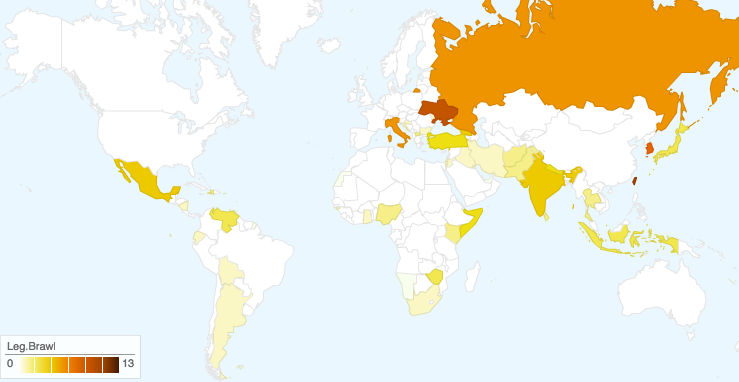
\includegraphics[width = 13cm]{incidence_map.png}
\end{figure}

%%%%%%%%%%%%%% Describing violence in National Legislatures
\section{Describing Violence in National Legislative Chambers Around the World (1981-2012)}

In order to further systematically explore the causes of legislative violence across the contemporary globe I primarily used the Google News Archive \citep{GoogleNews2011}, which has a global coverage of news sources, to create a data set of {\emph{physical fights between legislators in national legislative chambers}}.\footnote{The Google News Archive search was conducted in Spring 2011. A research assistant and I searched using terms that included `national' `parliament', `legislature', `assembly', `brawls', `scuffles', `fights'. This search was later supplemented in Spring 2013 by two other research assistants conducting Google and Youtube searches with these keywords.} This search was supplemented by information from colleagues resulting in a data set of \change{91}{116} incidents of legislative violence in 32 countries between 1981 and \change{Winter 2011}{2012}. We can see in Figure \ref{leg_map} that these events have occurred in many regions around the world. They do not appear to be confined to any one cultural group or region as a simple regional culture explanation would predict. Violence is nonetheless not evenly distributed across countries as we might expect if it was purely the result of legislators with violent personalities. Although I observed 32 countries having legislative violence, about 60 percent of these fights occurred in eight countries with four or more legislative brawls. These countries include Ukraine, Mexico, South Korea, and Taiwan.

Before moving on to the regression analysis it is useful to first examine the simple associations between proportional electoral outcomes, democratic age, and violence in this data. Figure \ref{framework_empirical} plots variables measuring these concepts in the entire sample of countries. In the following parametric analysis we will only look at multi-party elected legislatures. Each point represents a country-year. It's notable that virtually every observed incidence of violence took place in legislatures with more disproportionate seat distributions. Similarly, older democracies (approximately 55 years or older) were never observed having legislative brawls in the chamber. See below for details about how disproportionality and democratic age are measured.

While it appears that having disproportionate electoral outcomes \emph{or} a new democracy is not necessary for legislative violence, based on the data, having \emph{both} of them might make violence much more likely. South Korea's national assembly, like the antebellum US Senate, is an example of a `perfect storm'. It is both in a new democracy and has relatively disproportionate electoral outcomes.\footnote{South Korea’s average disproportionality as measured by the Gallagher Index \citep{Gallagher1991} from 2000 until 2011 was 12.7. This places it in the upper 25 percent of observations with elected legislatures. It also became a democracy within the past 20 years.} South Korea had eight observed incidence of legislative violence in the full sample. Countries that have \emph{either} proportional outcomes \emph{or} old democracies appear to be able to compensate fairly well for an absence of the other characteristic. The United Kingdom has a relatively disproportionate electoral system,\footnote{It had an average Gallagher disproportionality of 16.5 from 2000 to 2011.} but no violence in the sample. One reason for this might be that it has a very old democracy where the major parties have had experience in government and so view commitments to allow for the alteration of power to be credible. Conversely, only one incident of violence\footnote{Two members of parliament punched each other in 1998.} was observed in South Africa's new democracy. South Africa's democracy is about the same age as South Korea's and the country has a very violent recent past and present,\footnote{Its rate of murders per 100,000 people is regularly among the highest in the \cite{UNMurder2013} data set.} but it has very proportionate electoral outcomes.\footnote{South Africa’s average disproportionality was 0.29 from 2000 until 2011, one of the lowest observed in the sample.} South Africa's one scuffle in 1998 is quite an outlier as it is the only violent incident observed in very proportional legislatures in the sample.

This brief tour of descriptive statistics adds to the evidence from the previous case study suggesting that violence between legislators does not occur randomly or is confined to one cultural region. Instead violence does appear to be a characteristic of countries with disproportionate electoral outcomes and new democracies.

%%%%%%%%%%%%%%%% Scatterplot of Disproportionality, age_dem, and Violence %%%%%%%%%%%%%%%%%%%%%%%%
\begin{figure}[t]
    \caption{Scatter plots of Disproportionality, Age of Democracy, and Violence in the Full Sample.}
    \label{framework_empirical}
    \begin{center}

\begin{knitrout}
\definecolor{shadecolor}{rgb}{0.969, 0.969, 0.969}\color{fgcolor}\begin{kframe}


{\ttfamily\noindent\bfseries\color{errorcolor}{\#\# Error in eval(expr, envir, enclos): object 'dem\_age' not found}}\end{kframe}
\end{knitrout}
    \end{center}
    \begin{singlespace}
        {\scriptsize{Each point represents a country-year. The data is from a sample of 200 countries from 1981 through 2009 due to data availability. The points are jittered horizontally.}}
    \end{singlespace}

\end{figure}

%%%%%%%%%%%%%%%% Run Analyses %%%%%%%%%%%%%%%%%%%%%%%%






